\section{Algorithms for special universes}\label{sec:easy}

This section contains our algorithms.
Section~\ref{sec:easy-conn} reduces $\beta_0$, and $\beta_1$ of graphs, to dynamic connectivity.
Section~\ref{sec:easy-s3} maintains all Betti numbers of a subcomplex of a fixed triangulation of the $3$-sphere, and more generally of any fixed geometric complex in~$\R^3$, in $O(\log^2 n)$ amortized time per update; together with the lower bound for complexes in~$\R^4$ (Theorem~\ref{thm:r4}), this separates three from four dimensions.
Section~\ref{sec:easy-width} maintains every Betti number with polylogarithmically many field operations per update in the worst case when the boundary matrices of the universe have small width or when the Hasse diagram of the universe has bounded treewidth.

Throughout, $c(G)$ denotes the number of connected components of a graph~$G$.
A \emph{dynamic connectivity} structure maintains a graph on a fixed vertex set under edge insertions and deletions, and answers queries of the form ``are $u$ and $v$ connected?''
We use the deterministic structure of Holm, de Lichtenberg, and Thorup~\cite{HDT01}.
On a vertex set $V$ it is initialized without edges in $O(|V|\log|V|)$ time.
Afterwards, any sequence of $s$ edge updates takes $O(s\log^2|V|)$ time in total, and each query takes $O(\log|V|/\log\log|V|)$ time.
Such a structure also maintains $c(G)$.
Before inserting an edge $uv$ we ask whether $u$ and $v$ are connected, and we decrease $c(G)$ by one if they are not.
After deleting an edge $uv$ we ask the same question, and we increase $c(G)$ by one if they are not.

\subsection{Connected components}\label{sec:easy-conn}

For a simplicial complex $K$, let $G_0(K)$ be the graph with vertex set $K_0$ and edge set~$K_1$.
For every field $\F$, $\beta_0(K;\F)=c(G_0(K))$~\cite{Mun84}.

\begin{proposition}\label{prop:beta0}
Let $\cU$ be a universe with $n$ simplices.
There is a deterministic data structure that maintains a subcomplex $K\subseteq\cU$ under the simplex updates of Problem~\ref{prob:betti} and returns $\beta_0(K;\F)$, for every field~$\F$, with preprocessing time $O(n\log n)$, amortized update time $O(\log^2 n)$, and query time $O(1)$.
If $\dim\cU\le1$, the same data structure also returns $\beta_1(K;\F)$ in $O(1)$ time.
\end{proposition}

\begin{proof}
Let $G$ be the graph with vertex set $\cU_0$ and edge set $K_1$.
Both endpoints of an edge of $K$ lie in~$K$, so $G$ consists of $G_0(K)$ together with the $|\cU_0|-n_0(K)$ vertices of $\cU_0\setminus K_0$, which are isolated.
Hence
\[
  \beta_0(K;\F)=c(G_0(K))=c(G)-|\cU_0|+n_0(K).
\]
We store $n_0(K)$, $n_1(K)$, and~$c(G)$, and we keep $G$ in the structure of~\cite{HDT01} on the vertex set~$\cU_0$, initially without edges.
Inserting or deleting a vertex changes only $n_0(K)$: the precondition of $\Delete$ ensures that a deleted vertex has no incident edge in~$K$, so $G$ does not change.
Inserting or deleting an edge changes $n_1(K)$ and is one edge update of~$G$, which also updates $c(G)$ with one connectivity query.
Simplices of dimension at least two do not change~$G$.
So the preprocessing takes $O(n\log n)$ time, any sequence of $t$ updates takes $O(t\log^2n)$ time, and the formula above answers a query in $O(1)$ time.

If $\dim\cU\le1$, then $\bd_2=0$, and~\eqref{eq:betti-rank} gives $\rk\bd_1=n_0(K)-\beta_0(K)$ and therefore
\[
  \beta_1(K)=n_1(K)-n_0(K)+\beta_0(K).
\]
\end{proof}

The proof uses only the interface of the connectivity structure.
With the deterministic structure of Wulff-Nilsen~\cite{WN13}, the amortized update time becomes $O(\log^2 n/\log\log n)$.
With the randomized structure of Kapron, King, and Mountjoy~\cite{KKM13}, the update time becomes polylogarithmic in the worst case, and the answers inherit the Monte Carlo guarantee of~\cite{KKM13}; with the deterministic structure of Chuzhoy et al.~\cite{CGLNPS20}, it becomes $n^{o(1)}$ in the worst case.
For graph filtrations, Dey, Hou, and Parsa~\cite{DHP23} go further and update persistence diagrams, not only Betti numbers, under local changes in sublinear time.

Proposition~\ref{prop:beta0} is optimal up to a logarithmic factor, without any conjecture.
P\v{a}tra\c{s}cu and Demaine~\cite{PD06} proved that in the cell-probe model with cells of $\Theta(\log N)$ bits, every dynamic connectivity structure on $N$ vertices has amortized update time or query time $\Omega(\log N)$.
We take as universe the complete graph on these $N$ vertices, with $n=N+\binom N2$ simplices, and insert all vertices during preprocessing.
A connectivity query for two vertices $u$ and~$v$ then reduces to two updates and two queries of dynamic~$\beta_0$: query $\beta_0$, insert the edge $uv$ (if it is absent), query $\beta_0$ again, and delete the edge; the vertices are connected if and only if $\beta_0$ did not decrease.
Since $\log n=\Theta(\log N)$, every data structure for dynamic $\beta_0$ also has amortized update time or query time $\Omega(\log n)$ in this model.
By Lemma~\ref{lem:suspension}, the suspension shifts reduced homology by one degree, so $\beta_{p}(S^{p}K)=\beta_0(K)-1$ for every nonempty complex~$K$ and every $p\ge1$, where $S^p$ is the $p$-fold suspension of Section~\ref{sec:lower-amortized}. Since $K$ always contains all vertices, it is nonempty, and each update of $K$ costs $3^p$ updates of $S^pK$; hence the same unconditional bound holds for $\beta_p$ for every fixed $p\ge1$.

\subsection{Subcomplexes of the \texorpdfstring{$3$}{3}-sphere}\label{sec:easy-s3}

We write $\lVert K\rVert$ for the geometric realization of a simplicial complex~$K$~\cite{Mun84}; if $K$ is a subcomplex of~$T$, then $\lVert K\rVert$ is a subspace of~$\lVert T\rVert$.
A \emph{triangulation} of a topological space $Y$ is a simplicial complex $T$ such that $\lVert T\rVert$ is homeomorphic to~$Y$.

Let $T$ be a triangulation of the $3$-sphere~$S^3$.
We use three standard facts.
\begin{enumerate}[label=(T\arabic*)]
\item\label{it:s3-pure} Every simplex of $T$ is a face of a tetrahedron of~$T$, and $T$ has no simplex of dimension larger than three.
\item\label{it:s3-pseudo} Every triangle of $T$ is a facet of exactly two tetrahedra of~$T$.
\item\label{it:s3-sphere} For every field $\F$, $\beta_0(T;\F)=\beta_3(T;\F)=1$ and $\beta_1(T;\F)=\beta_2(T;\F)=0$.
\end{enumerate}
Facts~\ref{it:s3-pure} and~\ref{it:s3-pseudo} hold for every triangulation of a closed $3$-manifold~\cite{Mun84}.
Fact~\ref{it:s3-sphere} holds because simplicial homology is a topological invariant~\cite{Mun84,Hat02}.
For a triangle $t$ of $T$, let $\tau_t$ and $\tau'_t$ be the two tetrahedra that contain~$t$.
Figure~\ref{fig:duality} shows the idea of this subsection one dimension lower.

% Figure: the duality behind the algorithm for subcomplexes of the 3-sphere, shown one dimension lower.
% Requires only tikz. The dual-graph coordinates were generated by a short script (components computed, not drawn by hand).
\begin{figure}[t]
\centering
\providecommand\Description[2][]{}%
\Description{A large triangle subdivided into sixteen small triangles. A thick black hexagon surrounds one vertex and a filled triangle sits at the top corner. Blue dots and edges connect the six triangles inside the hexagon; green dots and edges connect the triangles outside, with dashed green stubs leading out to the outer face.}
\definecolor{duA}{HTML}{0072B2}%
\definecolor{duB}{HTML}{009E73}%
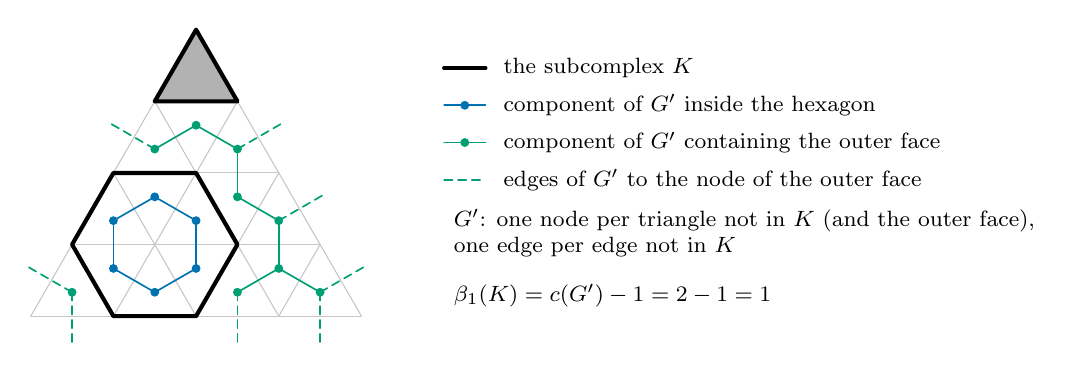
\begin{tikzpicture}[x=1.05cm,y=1.05cm,line join=round,line cap=round]
  % the triangulation T of a big triangle of side 4 (together with the outer face, a triangulated 2-sphere)
  \foreach \j in {0,...,3} {
    \pgfmathtruncatemacro{\m}{3-\j}
    \foreach \i in {0,...,\m} {
      \draw[black!22,line width=0.4pt] ({\i+0.5*\j},{0.866*\j}) -- ({\i+1+0.5*\j},{0.866*\j});
      \draw[black!22,line width=0.4pt] ({\i+0.5*\j},{0.866*\j}) -- ({\i+0.5*(\j+1)},{0.866*(\j+1)});
      \draw[black!22,line width=0.4pt] ({\i+1+0.5*\j},{0.866*\j}) -- ({\i+0.5*(\j+1)},{0.866*(\j+1)});
    }}
  % the filled triangle of K
  \fill[black!30] (1.5,2.598) -- (2.5,2.598) -- (2,3.464) -- cycle;
  % the graph G': nodes = triangles not in K, edges = edges not in K; dashed stubs lead to the outer face
\draw[duA,line width=0.6pt] (1.000,0.577) -- (1.500,0.289);
\draw[duA,line width=0.6pt] (1.000,0.577) -- (1.000,1.155);
\draw[duA,line width=0.6pt] (1.500,0.289) -- (2.000,0.577);
\draw[duA,line width=0.6pt] (2.000,0.577) -- (2.000,1.155);
\draw[duB,line width=0.6pt] (2.500,0.289) -- (3.000,0.577);
\draw[duB,line width=0.6pt] (3.000,0.577) -- (3.500,0.289);
\draw[duB,line width=0.6pt] (3.000,0.577) -- (3.000,1.155);
\draw[duA,line width=0.6pt] (1.000,1.155) -- (1.500,1.443);
\draw[duA,line width=0.6pt] (1.500,1.443) -- (2.000,1.155);
\draw[duB,line width=0.6pt] (2.500,1.443) -- (3.000,1.155);
\draw[duB,line width=0.6pt] (2.500,1.443) -- (2.500,2.021);
\draw[duB,line width=0.6pt] (1.500,2.021) -- (2.000,2.309);
\draw[duB,line width=0.6pt] (2.000,2.309) -- (2.500,2.021);
\draw[duB,line width=0.6pt,densely dashed] (0.500,0.289) -- (0.500,-0.320);
\draw[duB,line width=0.6pt,densely dashed] (0.500,0.289) -- (-0.027,0.593);
\draw[duB,line width=0.6pt,densely dashed] (2.500,0.289) -- (2.500,-0.320);
\draw[duB,line width=0.6pt,densely dashed] (3.500,0.289) -- (3.500,-0.320);
\draw[duB,line width=0.6pt,densely dashed] (3.500,0.289) -- (4.027,0.593);
\draw[duB,line width=0.6pt,densely dashed] (3.000,1.155) -- (3.527,1.459);
\draw[duB,line width=0.6pt,densely dashed] (1.500,2.021) -- (0.973,2.325);
\draw[duB,line width=0.6pt,densely dashed] (2.500,2.021) -- (3.027,2.325);
\fill[duB] (0.500,0.289) circle (1.6pt);
\fill[duA] (1.000,0.577) circle (1.6pt);
\fill[duA] (1.500,0.289) circle (1.6pt);
\fill[duA] (2.000,0.577) circle (1.6pt);
\fill[duB] (2.500,0.289) circle (1.6pt);
\fill[duB] (3.000,0.577) circle (1.6pt);
\fill[duB] (3.500,0.289) circle (1.6pt);
\fill[duA] (1.000,1.155) circle (1.6pt);
\fill[duA] (1.500,1.443) circle (1.6pt);
\fill[duA] (2.000,1.155) circle (1.6pt);
\fill[duB] (2.500,1.443) circle (1.6pt);
\fill[duB] (3.000,1.155) circle (1.6pt);
\fill[duB] (1.500,2.021) circle (1.6pt);
\fill[duB] (2.000,2.309) circle (1.6pt);
\fill[duB] (2.500,2.021) circle (1.6pt);

  % K: a hexagonal 1-cycle and a filled triangle
  \draw[black,line width=1.5pt] (2,0) -- (2.5,0.866) -- (2,1.732) -- (1,1.732) -- (0.5,0.866) -- (1,0) -- cycle;
  \draw[black,line width=1.5pt] (1.5,2.598) -- (2.5,2.598) -- (2,3.464) -- cycle;
  % legend
  \begin{scope}[shift={(5.0,3.0)},font=\footnotesize]
    \draw[black,line width=1.5pt] (0,0) -- (0.5,0); \node[anchor=west] at (0.6,0) {the subcomplex $K$};
    \draw[duA,line width=0.6pt] (0,-0.45) -- (0.5,-0.45); \fill[duA] (0.25,-0.45) circle (1.6pt);
    \node[anchor=west] at (0.6,-0.45) {component of $G'$ inside the hexagon};
    \draw[duB,line width=0.6pt] (0,-0.9) -- (0.5,-0.9); \fill[duB] (0.25,-0.9) circle (1.6pt);
    \node[anchor=west] at (0.6,-0.9) {component of $G'$ containing the outer face};
    \draw[duB,line width=0.6pt,densely dashed] (0,-1.35) -- (0.5,-1.35);
    \node[anchor=west] at (0.6,-1.35) {edges of $G'$ to the node of the outer face};
    \node[anchor=west,align=left] at (0,-2.0) {$G'$: one node per triangle not in $K$ (and the outer face),\\one edge per edge not in $K$};
    \node[anchor=west] at (0,-2.75) {$\beta_1(K)=c(G')-1=2-1=1$};
  \end{scope}
\end{tikzpicture}
\caption{The duality behind Theorem~\ref{thm:s3}, one dimension lower.
For a proper subcomplex $K$ of a triangulated $2$-sphere, of which only a triangulated disk is drawn (the triangles outside the disk are not in~$K$ and are merged into one node, the outer face), Alexander duality gives $\beta_1(K)=c-1$, where $c$ is the number of components of the complement of~$K$, and these components are the components of the graph~$G'$ whose nodes are the triangles not in~$K$ (and the outer face) and whose edges are the edges not in~$K$, as in the proof of Lemma~\ref{lem:dual}.
A simplex update changes $G'$ by $O(1)$ nodes or edges, so dynamic connectivity maintains~$\beta_1(K)$.
For a triangulated $3$-sphere, the same argument applies to $\beta_2$, with tetrahedra as nodes and triangles as edges.}
\label{fig:duality}
\end{figure}


\begin{definition}[Dual graph]
For a subcomplex $K\subseteq T$, the \emph{dual graph} $G_\ast(K)$ has the set $T_3$ of all tetrahedra of $T$ as its vertex set and, for every triangle $t\in T_2\setminus K$, an edge $t^\ast$ that joins $\tau_t$ and~$\tau'_t$.
\end{definition}

The graph $G_\ast(K)$ is simple, because two tetrahedra that share two triangles share all four vertices.
A tetrahedron of $K$ is an isolated vertex of $G_\ast(K)$, because all its triangles lie in~$K$.

\begin{lemma}\label{lem:dual}
Let $T$ be a triangulation of $S^3$, let $\F$ be a field, and let $K\subsetneq T$ be a subcomplex.
Then
\[
  \beta_3(K;\F)=0\qquad\text{and}\qquad\beta_2(K;\F)=c(G_\ast(K))-n_3(K)-1.
\]
\end{lemma}

\begin{proof}
We fix an orientation of every tetrahedron and write $[\tau:t]\in\{1,-1\}$ for the coefficient of a triangle $t$ in $\bd\tau$.
By~\ref{it:s3-pseudo}, for every $3$-chain $c=\sum_{\tau}c_\tau\tau$ and every triangle~$t$,
\begin{equation}\label{eq:dual-coef}
  \text{the coefficient of $t$ in $\bd c$ is } [\tau_t:t]\,c_{\tau_t}+[\tau'_t:t]\,c_{\tau'_t}.
\end{equation}

\emph{Step 1: $G_\ast(\emptyset)$ is connected, and the orientations can be chosen so that $[\tau'_t:t]=-[\tau_t:t]$ for every triangle~$t$.}
Over $\Ftwo$, \eqref{eq:dual-coef} shows that a $3$-chain is a cycle if and only if its coefficients agree at the two endpoints of every edge of $G_\ast(\emptyset)$.
So $\dim Z_3(T;\Ftwo)=c(G_\ast(\emptyset))$.
Since $T$ has no $4$-simplices by~\ref{it:s3-pure}, $\dim Z_3(T;\Ftwo)=\beta_3(T;\Ftwo)$, which is $1$ by~\ref{it:s3-sphere}.
Hence $G_\ast(\emptyset)$ is connected.
Over $\mathbb{Q}$, fact~\ref{it:s3-sphere} provides a cycle $z\ne0$ in $Z_3(T;\mathbb{Q})$.
By~\eqref{eq:dual-coef}, $|z_{\tau_t}|=|z_{\tau'_t}|$ for every triangle~$t$.
Since $G_\ast(\emptyset)$ is connected, all coefficients of $z$ have the same absolute value $\alpha$, and $\alpha>0$ because $z\ne0$.
We reverse the orientation of every tetrahedron $\tau$ with $z_\tau<0$.
Then $z=\alpha\sum_\tau\tau$, and~\eqref{eq:dual-coef} applied to $z$ gives $[\tau_t:t]+[\tau'_t:t]=0$ for every triangle~$t$.
These are integers, so the identity holds over every field.
From now on we use these orientations.
Then~\eqref{eq:dual-coef} says that the coefficient of $t$ in $\bd c$ is $[\tau_t:t]\,(c_{\tau_t}-c_{\tau'_t})$.

\emph{Step 2: $\beta_3(K)=0$.}
By Step~1, every $3$-cycle of $T$ has equal coefficients at the two endpoints of every edge of the connected graph $G_\ast(\emptyset)$, so it has the same coefficient on all tetrahedra.
If $K$ contained every tetrahedron of $T$, then $K$ would contain all their faces, and $K=T$ by~\ref{it:s3-pure}.
So some tetrahedron is not in~$K$.
A $3$-cycle of $K$ is a $3$-cycle of $T$ with coefficient zero on that tetrahedron, so it is zero.
Since $K$ has no $4$-simplices, $\beta_3(K)=\dim Z_3(K)=0$.

\emph{Step 3: $\beta_2(K)$.}
The relative chain groups $C_q(T,K)=C_q(T)/C_q(K)$ have the simplices of $T_q\setminus K_q$ as a basis.
The exact sequence of the pair $(T,K)$~\cite{Mun84} contains the segment
\[
  H_3(K)\to H_3(T)\to H_3(T,K)\to H_2(K)\to H_2(T).
\]
Here $H_3(K)=0$ by Step~2, $H_3(T)\cong\F$ and $H_2(T)=0$ by~\ref{it:s3-sphere}, so $\beta_2(K)=\dim H_3(T,K)-1$.
Since $T$ has no $4$-simplices, $H_3(T,K)$ is the space of relative $3$-cycles: chains $c$ on the tetrahedra not in $K$ such that $\bd c$ has coefficient zero on every triangle $t\notin K$.
For such a triangle, $\tau_t$ and $\tau'_t$ are not in $K$, because $K$ is closed under taking faces.
By Step~1, the condition for $t$ says $c_{\tau_t}=c_{\tau'_t}$.
Let $G'$ be the subgraph of $G_\ast(K)$ induced by $T_3\setminus K_3$; it contains every edge of $G_\ast(K)$.
The relative $3$-cycles are exactly the chains that are constant on every connected component of~$G'$, so $\dim H_3(T,K)=c(G')$.
The tetrahedra of $K$ are isolated vertices of $G_\ast(K)$, so $c(G')=c(G_\ast(K))-n_3(K)$.
\end{proof}

\begin{theorem}\label{thm:s3}
Let $T$ be a triangulation of $S^3$ with $n$ simplices.
There is a deterministic data structure that maintains a subcomplex $K\subseteq T$ under the simplex updates of Problem~\ref{prob:betti} with universe $\cU=T$, and that returns $\beta_0(K;\F),\dots,\beta_3(K;\F)$, for every field $\F$, in $O(1)$ time.
The preprocessing and any sequence of $t$ updates take $O((n+t)\log^2n)$ time in total.
\end{theorem}

\begin{proof}
The data structure stores the counters $n_0(K),\dots,n_3(K)$ and two dynamic connectivity structures~\cite{HDT01} that maintain their numbers of components.
The first, $\mathcal{D}_0$, stores the graph $G$ with vertex set $T_0$ and edge set $K_1$, as in the proof of Proposition~\ref{prop:beta0}.
The second, $\mathcal{D}_\ast$, stores the dual graph $G_\ast(K)$.
In preprocessing we compute $\tau_t$ and $\tau'_t$ for every triangle $t$ by sorting the triangles of all tetrahedra, in $O(n\log n)$ time.
We initialize both structures, and we insert the $n_2(T)\le n$ edges of $G_\ast(\emptyset)$ into~$\mathcal{D}_\ast$.

An update of a vertex or of a tetrahedron changes only the corresponding counter.
An update of an edge also inserts or deletes that edge in~$\mathcal{D}_0$.
Inserting a triangle into $K$ deletes its dual edge from~$\mathcal{D}_\ast$, and deleting a triangle from $K$ inserts its dual edge.
So every update costs $O(1)$ time plus at most one edge update and one connectivity query in one of the two structures.
Both structures have at most $n$ vertices.
After their initialization, they receive at most $n+t$ edge updates and $t$ queries in total, so the preprocessing and $t$ updates take $O(n\log n+(n+t)\log^2n+t\log n)=O((n+t)\log^2n)$ time.

To answer a query, we distinguish two cases.
If $n_3(K)=n_3(T)$, then $K$ contains every tetrahedron, so $K=T$ by~\ref{it:s3-pure}, and we return $(1,0,0,1)$, which is correct by~\ref{it:s3-sphere}.
Otherwise $K\subsetneq T$, and we return
\[
  \beta_0=c(G)-n_0(T)+n_0(K),\quad \beta_2=c(G_\ast(K))-n_3(K)-1,\quad \beta_3=0,\quad \beta_1=\beta_0+\beta_2-\beta_3-\chi(K),
\]
where $\chi(K)=n_0(K)-n_1(K)+n_2(K)-n_3(K)$.
The value $\beta_0$ is correct by the proof of Proposition~\ref{prop:beta0}, $\beta_2$ and $\beta_3$ are correct by Lemma~\ref{lem:dual}, and $\beta_1$ is then correct by the Euler--Poincar\'e formula $\chi(K)=\sum_p(-1)^p\beta_p(K)$ of Section~\ref{sec:prelim}.
None of these values depends on~$\F$, and each is computed from stored numbers in $O(1)$ time.
\end{proof}

Thus, after preprocessing, any $t$ updates take $O((n+t)\log^2 n)$ time, which is amortized update time $O(\log^2 n)$ in the sense of Section~\ref{sec:prelim}; the term $n\log^2n$ pays for the potential that the $n_2(T)$ initial edges of $\mathcal{D}_\ast$ create in the analysis of~\cite{HDT01}.
With~\cite{WN13} the total time becomes $O((n+t)\log^2n/\log\log n)$, with the randomized (Monte Carlo) structure of~\cite{KKM13} every update takes polylogarithmic worst-case time, and with the deterministic structure of~\cite{CGLNPS20} every update takes $n^{o(1)}$ worst-case time.
The formulas show that the Betti numbers of a subcomplex of $T$ do not depend on the field.

Lemma~\ref{lem:dual} is a combinatorial form of Alexander duality.
Identify $\lVert T\rVert$ with $S^3$ and let $\emptyset\ne K\subsetneq T$; then $\widetilde H_0(S^3\setminus\lVert K\rVert;\Z)\cong\widetilde H^2(\lVert K\rVert;\Z)$~\cite[Section~3.3]{Hat02}, the right-hand side has rank $\beta_2(K;\mathbb{Q})$ by the universal coefficient theorem, and so $c(G_\ast(K))-n_3(K)$ is the number of path components of $S^3\setminus\lVert K\rVert$.
We do not use this fact.
Delfinado and Edelsbrunner~\cite{DE95} use the same two graphs to compute the Betti numbers of a filtration of a subcomplex of a triangulated $S^3$ in $O(n\,\alpha(n))$ time, where $\alpha$ is the inverse Ackermann function.
Since union--find cannot delete, they process the dual graph in reverse order.
Fully dynamic connectivity removes this restriction, so in Theorem~\ref{thm:s3} insertions and deletions can arrive in any order.
In their Section~6.2 they also drop the triangulation of the complement and handle every complex in~$\R^3$ through a graph on the two sides of its triangles, built from the cyclic order of the triangles around each edge; Corollary~\ref{cor:anyR3} below obtains the dynamic version more simply, at the price of polynomial preprocessing.

The same algorithm applies to subcomplexes of a triangulated $3$-ball.

\begin{corollary}\label{cor:r3}
Let $B$ be a triangulation of the closed $3$-ball with $n_B$ simplices, and let the universe $\cU$ be a subcomplex of~$B$.
There is a deterministic data structure that maintains a subcomplex $K\subseteq\cU$ under the simplex updates of Problem~\ref{prob:betti} and returns $\beta_0(K;\F),\dots,\beta_3(K;\F)$, for every field $\F$, in $O(1)$ time.
The preprocessing and any sequence of $t$ updates take $O((n_B+t)\log^2n_B)$ time in total.
\end{corollary}

\begin{proof}
Let $\bd B$ be the set of triangles of $B$ that are facets of exactly one tetrahedron of~$B$, together with all their faces.
It is a subcomplex of~$B$, and $\lVert\bd B\rVert$ is the boundary sphere of the ball $\lVert B\rVert$~\cite{Mun84}.
Let $o$ be a new vertex, let $C=\{\{o\}\}\cup\bd B\cup\{\sigma\cup\{o\}:\sigma\in\bd B\}$ be the cone on $\bd B$ with apex~$o$, and let $T=B\cup C$.
Then $T$ is a simplicial complex with at most $2n_B+1$ simplices, $B\cap C=\bd B$, and $\lVert C\rVert$ is a cone on $\lVert\bd B\rVert$.
So $\lVert T\rVert$ is the union of the ball $\lVert B\rVert$ and a cone on its boundary sphere, and the two meet exactly in that sphere.
A homeomorphism from $\lVert B\rVert$ to the closed unit ball $D^3\subset\R^3$ maps the boundary sphere $\lVert\bd B\rVert$ onto the unit sphere $S^2$, and it extends along the cone lines to a homeomorphism from $\lVert T\rVert$ to the space obtained from $D^3$ by attaching a cone on~$S^2$ along~$S^2$.
The cone on $S^2$ is a closed $3$-ball, and two closed $3$-balls glued along their boundary spheres by a homeomorphism form $S^3$, so $T$ is a triangulation of~$S^3$.
We compute $\bd B$ and $T$ in $O(n_B\log n_B)$ time.
Every subcomplex of $\cU$ is a subcomplex of~$T$, and the preconditions of $\Insert$ and $\Delete$ depend only on $K$ and on the updated simplex.
So the data structure of Theorem~\ref{thm:s3} for $T$ solves the problem for~$\cU$.
\end{proof}

A compact convex set in $\R^3$ with nonempty interior is homeomorphic to the closed $3$-ball.
So Corollary~\ref{cor:r3} applies to every subcomplex of a geometric simplicial complex in $\R^3$ whose underlying space is a $3$-dimensional convex polytope.
An example is the Delaunay triangulation of a finite set of at least four points in general position in~$\R^3$, whose subcomplexes include the alpha complexes of the point set~\cite{EH10}.

In fact, polynomial preprocessing suffices to handle every fixed geometric complex in~$\R^3$, with no assumption on its underlying space.

\begin{corollary}\label{cor:anyR3}
Let $\cU$ be a geometric simplicial complex in $\R^3$ with $n$ simplices, given by rational vertex coordinates.
There is a deterministic data structure that maintains a subcomplex $K\subseteq\cU$ under the simplex updates of Problem~\ref{prob:betti} and returns $\beta_0(K;\F),\dots,\beta_3(K;\F)$, for every field~$\F$, in $O(1)$ time.
Its preprocessing time is polynomial in the size of the input, and afterwards any sequence of $t$ updates takes $O((n+t)\log^2n)$ time in total.
\end{corollary}

\begin{proof}
\emph{A refinement.}
Fix a closed tetrahedron $\Delta\subset\R^3$ whose interior contains $\lVert\cU\rVert$.
Cut $\Delta$ by the planes spanned by the triangles of~$\cU$ and, for every edge and every vertex of $\cU$, by two or three planes through it whose intersection is exactly the line or point that it spans.
Every simplex of $\cU$ is then a union of closed cells, of all dimensions, of the resulting decomposition of $\Delta$ into convex polytopes, and the barycentric subdivision of this decomposition is a triangulation $B$ of $\Delta$ in which every simplex of $\cU$ is a union of simplices of~$B$~\cite{Mun84}.
There are $O(n)$ planes, so $B$ has polynomially many simplices and can be computed in polynomial time.
Coning off $\bd B$ as in the proof of Corollary~\ref{cor:r3} gives a triangulation $T$ of $S^3$ with the same property.
For a subcomplex $K\subseteq\cU$, the simplices of $T$ contained in $\lVert K\rVert$ form a subcomplex $K'\subsetneq T$ with $\lVert K'\rVert=\lVert K\rVert$, so $K$ and $K'$ have the same Betti numbers.
By Lemma~\ref{lem:dual}, $\beta_3(K)=0$ and $\beta_2(K)=c(G_\ast(K'))-n_3(K')-1$, where $G_\ast$ is the dual graph of~$T$.

\emph{A compressed dual graph.}
We call the connected components of $S^3\setminus\lVert\cU\rVert$ the \emph{outer cells}.
Near an interior point of a triangle $t$ of $\cU$, no simplex of $\cU$ other than $t$ and the tetrahedra that contain $t$ is present, so each of the two sides of $t$ lies in a single outer cell or in a single tetrahedron of $\cU$ that contains~$t$.
Let $G(K)$ be the multigraph whose nodes are the outer cells and the tetrahedra of $\cU$, with one edge for every triangle $t\in\cU_2\setminus K$, joining the nodes on the two sides of~$t$.
We claim that $c(G_\ast(K'))-n_3(K')=c(G(K))-n_3(K)$.
The interior of every tetrahedron of $T$ lies in an outer cell or in the interior of a tetrahedron of~$\cU$.
The tetrahedra of $T$ in one outer cell are connected in $G_\ast(K')$: a path between two of them inside the open cell can be chosen to avoid the $1$-skeleton of $T$ and to cross triangles of $T$ transversally, and the triangles that it crosses lie inside the cell, so they are not in~$K'$.
For a tetrahedron $\tau\in\cU_3\setminus K$, the tetrahedra of $T$ in $\tau$ are connected through the triangles of $T$ in the interior of~$\tau$, which are not in~$K'$; for $\tau\in K$, each of them is an isolated vertex of $G_\ast(K')$, and it is also counted in $n_3(K')$.
A triangle of $T$ that is contained in a triangle $t$ of $\cU$ lies in $K'$ if and only if $t\in K$, because $\lVert K\rVert\cap\lVert t\rVert$ is a union of faces of~$t$; if $t\notin K$, it joins tetrahedra of $T$ on the two sides of~$t$.
The relative interior of every other triangle of $T$ lies in an outer cell or in the interior of a tetrahedron of~$\cU$.
Contracting the groups of tetrahedra of $T$ described above therefore turns $G_\ast(K')$ into $G(K)$, up to the multiplicity of edges (a triangle $t\notin K$ of $\cU$ yields one edge for each triangle of $T$ inside~$t$, which does not affect connectivity), except that a tetrahedron $\tau\in K$ of $\cU$ corresponds to its $T$-tetrahedra, which are isolated in $G_\ast(K')$ and counted in $n_3(K')$, while in $G(K)$ it is a single isolated node counted in $n_3(K)$.
This proves the claim, so $\beta_2(K)=c(G(K))-n_3(K)-1$.

\emph{The data structure.}
In preprocessing we compute $T$, the outer cells, and the two sides of every triangle of~$\cU$.
The multigraph $G(K)$ has at most $n_3(\cU)+2n_2(\cU)+1$ nodes and at most $n$ edges.
We then proceed as in the proof of Theorem~\ref{thm:s3}, with a dynamic connectivity structure for $G(K)$ in place of $\mathcal{D}_\ast$; parallel edges and loops are handled by keeping a multiplicity for every pair of nodes.
A simplex update of $K$ changes at most one edge of $G(K)$ or of $G_0(K)$, so it takes $O(\log^2n)$ amortized time, and the query formulas are those of Theorem~\ref{thm:s3} with $c(G(K))$ in place of $c(G_\ast(K))$; the case $K=T$ does not occur.
\end{proof}

\paragraph{Three versus four dimensions.}
Theorem~\ref{thm:s3}, Corollary~\ref{cor:anyR3}, and Theorem~\ref{thm:r4} separate three from four dimensions.
For subcomplexes of any fixed geometric complex in $\R^3$, all Betti numbers can be maintained in $O(\log^2 n)$ amortized time per update after polynomial preprocessing; preprocessing and $t$ updates take $O((n+t)\log^2 n)$ time in total if the universe is a triangulation of the $3$-sphere (Theorem~\ref{thm:s3}), and $O((n_B+t)\log^2 n_B)$ time if it is a subcomplex of a given triangulated $3$-ball with $n_B$ simplices (Corollary~\ref{cor:r3}).
For subcomplexes of a fixed geometric $2$-complex in $\R^4$, no data structure with polynomial preprocessing time maintains $\beta_1$ or $\beta_2$ with amortized update time $O(n^{1/2-\eps})$ and query time $O(n^{1-\eps})$, unless the \OMv\ conjecture fails (Theorem~\ref{thm:r4}).
Duality explains where the boundary lies.
The proof of Lemma~\ref{lem:dual} works verbatim for a triangulation $T$ of the $d$-sphere with $d\ge2$: for every proper subcomplex $K$, $\beta_d(K)=0$ and $\beta_{d-1}(K)=c(G_\ast(K))-n_d(K)-1$, where $G_\ast(K)$ joins two $d$-simplices through every $(d-1)$-simplex not in~$K$.
With dynamic connectivity for $\beta_0$ and the Euler--Poincar\'e formula, this determines all Betti numbers if $d\le3$, because at most one Betti number, $\beta_1$, remains unknown.
For $d=4$, two Betti numbers remain, $\beta_1$ and $\beta_2$, tied by a single linear relation; these are exactly the Betti numbers for which Theorem~\ref{thm:r4} proves hardness in~$\R^4$.
This is the dynamic counterpart of the static picture: Betti numbers of subcomplexes of a triangulated $S^3$ can be computed in near-linear time~\cite{DE95}, Dey and Guha~\cite{DG98} compute the homology groups of complexes in~$\R^3$, and for $2$-complexes that embed in $\R^4$ the problem is as hard as matrix rank~\cite{EP14}.
By Corollary~\ref{cor:anyR3}, both sides live in the same model: the universe is a fixed geometric complex, and preprocessing may take polynomial time.
Whether the lower bound holds for subcomplexes of a triangulation of the $4$-sphere with $O(n)$ simplices is open (Section~\ref{sec:conclusion}).

\subsection{Small width and bounded treewidth}\label{sec:easy-width}

Let $\F$ be a field and $M\in\F^{r\times k}$.
We count field operations as unit cost.
We consider dynamic rank under column switches only: the data structure maintains a set $J\subseteq[k]$ of active columns, initially empty, under $\Toggle(\text{column }j)$, and $\Query$ returns $\rk M[[r],J]$.
By Lemma~\ref{lem:betti-to-rank}, this problem captures dynamic Betti numbers: the columns of a boundary matrix are the simplices of one dimension, and a simplex update switches one column.
Zero rows and zero columns do not affect the rank.
So we delete them in preprocessing, ignore switches of zero columns, and assume that every row and every column of $M$ is nonzero.
For a set $S$ of rows, $\pi_S\colon\F^r\to\F^S$ denotes the coordinate projection, $m_j$ denotes column $j$ of~$M$, and $\nnz(M)$ is the number of nonzero entries of~$M$.

\paragraph{Column hierarchies.}
A \emph{column hierarchy} for $M$ is a rooted tree $H$ whose leaves are the columns $1,\dots,k$ and in which every inner node has one or two children.
Its \emph{height} is the largest number of edges on a path from the root to a leaf.
For a node $\theta$ of $H$, let $L_\theta\subseteq[k]$ be the set of columns at the leaves below~$\theta$, so that $L_\theta=\{j\}$ if $\theta$ is the leaf~$j$.
Let $\operatorname{In}(\theta)$ be the set of rows all of whose nonzero entries lie in columns of~$L_\theta$, and let $\operatorname{Bd}(\theta)$ be the set of rows that have a nonzero entry in a column of $L_\theta$ and a nonzero entry in a column outside~$L_\theta$.
The \emph{width} of $H$ is the largest size of a set $\operatorname{Bd}(\theta)$.
Contracting an inner node that has a single child into that child changes neither the sets $L_\theta$ that occur nor the width, and it does not increase the height; so we may assume that every inner node has two children, and then $H$ has fewer than $2k$ nodes.

\begin{theorem}\label{thm:hier}
Let $\F$ be a field, let $M\in\F^{r\times k}$, and let $H$ be a column hierarchy for $M$ of height $h$ and width~$w$.
There is a deterministic data structure for dynamic rank of $M$ under column switches with preprocessing time $O(r+k+\nnz(M)(h+1))$, worst-case update time $O((w+1)^3(h+1))$, and query time $O(1)$.
\end{theorem}

For a node $\theta$, let $V_\theta\subseteq\F^r$ be the span of the active columns in~$L_\theta$, let $r_\theta=\dim\pi_{\operatorname{In}(\theta)}(V_\theta)$, and let $W_\theta=\{v\in V_\theta:\pi_{\operatorname{In}(\theta)}(v)=0\}$.
If a column of $L_\theta$ has a nonzero entry in row~$i$, then $i\in\operatorname{In}(\theta)\cup\operatorname{Bd}(\theta)$.
So every vector of $V_\theta$ is supported on $\operatorname{In}(\theta)\cup\operatorname{Bd}(\theta)$, and every vector of $W_\theta$ is supported on $\operatorname{Bd}(\theta)$.
By the rank--nullity theorem, $\dim V_\theta=r_\theta+\dim W_\theta$.
At the root $\rho$, every row lies in $\operatorname{In}(\rho)$, so $W_\rho=0$ and $\rk M[[r],J]=\dim V_\rho=r_\rho$.

\begin{lemma}\label{lem:merge}
Let $\theta$ be a node of $H$ with children $\theta_1$ and~$\theta_2$, and let $X=\operatorname{In}(\theta)\setminus(\operatorname{In}(\theta_1)\cup\operatorname{In}(\theta_2))$.
\begin{enumerate}[label=(\alph*)]
\item $X\subseteq\operatorname{Bd}(\theta_1)\cap\operatorname{Bd}(\theta_2)$; in particular $|X|\le w$.
\item The set $\operatorname{Bd}(\theta_1)\cup\operatorname{Bd}(\theta_2)$ is the disjoint union of $\operatorname{Bd}(\theta)$ and~$X$.
\item $r_\theta=r_{\theta_1}+r_{\theta_2}+\dim\pi_X(W_{\theta_1}+W_{\theta_2})$ and $W_\theta=\{v\in W_{\theta_1}+W_{\theta_2}:\pi_X(v)=0\}$.
\end{enumerate}
\end{lemma}

\begin{proof}
(a)~A row of $X$ has all its nonzero entries in $L_\theta=L_{\theta_1}\sqcup L_{\theta_2}$, but neither all in $L_{\theta_1}$ nor all in~$L_{\theta_2}$.
So it has a nonzero entry in each of $L_{\theta_1}$ and $L_{\theta_2}$, and it lies in $\operatorname{Bd}(\theta_1)$ and in $\operatorname{Bd}(\theta_2)$.

(b)~A row of $\operatorname{Bd}(\theta)$ has a nonzero entry in $L_\theta$, hence in $L_{\theta_1}$ or in~$L_{\theta_2}$, and a nonzero entry outside $L_\theta$, hence outside both; so it lies in $\operatorname{Bd}(\theta_1)\cup\operatorname{Bd}(\theta_2)$.
By~(a), so does every row of~$X$.
Conversely, let $i\in\operatorname{Bd}(\theta_1)$; the case of $\theta_2$ is symmetric.
If $i$ has a nonzero entry outside $L_\theta$, then $i\in\operatorname{Bd}(\theta)$.
Otherwise $i\in\operatorname{In}(\theta)$; moreover $i\notin\operatorname{In}(\theta_1)$ because $i\in\operatorname{Bd}(\theta_1)$, and $i\notin\operatorname{In}(\theta_2)$ because $i$ has a nonzero entry in~$L_{\theta_1}$; so $i\in X$.
The sets $\operatorname{Bd}(\theta)$ and $X$ are disjoint, because $X\subseteq\operatorname{In}(\theta)$.

(c)~Let $Y=\operatorname{In}(\theta_1)\cup\operatorname{In}(\theta_2)$; this is a disjoint union, and $\operatorname{In}(\theta)=Y\cup X$.
The rows of $\operatorname{In}(\theta_1)$ have all their nonzero entries in $L_{\theta_1}$, so every vector of $V_{\theta_2}$ vanishes on them; symmetrically, every vector of $V_{\theta_1}$ vanishes on $\operatorname{In}(\theta_2)$.
We have $V_\theta=V_{\theta_1}+V_{\theta_2}$.
For $v_1\in V_{\theta_1}$ and $v_2\in V_{\theta_2}$, therefore, $\pi_{\operatorname{In}(\theta_1)}(v_1+v_2)=\pi_{\operatorname{In}(\theta_1)}(v_1)$ and $\pi_{\operatorname{In}(\theta_2)}(v_1+v_2)=\pi_{\operatorname{In}(\theta_2)}(v_2)$.
Hence $\pi_Y(V_\theta)$ is the direct sum of $\pi_{\operatorname{In}(\theta_1)}(V_{\theta_1})$ and $\pi_{\operatorname{In}(\theta_2)}(V_{\theta_2})$, of dimension $r_{\theta_1}+r_{\theta_2}$.
Moreover, $\pi_Y(v_1+v_2)=0$ if and only if $v_1\in W_{\theta_1}$ and $v_2\in W_{\theta_2}$, so the kernel of $\pi_Y$ on $V_\theta$ is $W_{\theta_1}+W_{\theta_2}$.
It follows that $\dim V_\theta=r_{\theta_1}+r_{\theta_2}+\dim(W_{\theta_1}+W_{\theta_2})$, and that $W_\theta$, the kernel of $\pi_{\operatorname{In}(\theta)}$ on $V_\theta$, consists of the vectors $v\in W_{\theta_1}+W_{\theta_2}$ with $\pi_X(v)=0$.
By rank--nullity for $\pi_X$ on $W_{\theta_1}+W_{\theta_2}$, we get $r_\theta=\dim V_\theta-\dim W_\theta=r_{\theta_1}+r_{\theta_2}+\dim\pi_X(W_{\theta_1}+W_{\theta_2})$.
\end{proof}

\begin{proof}[Proof of Theorem~\ref{thm:hier}]
We assume that every inner node of $H$ has two children.
At each node $\theta$ we store the number $r_\theta$ and a basis of $W_\theta$, written as vectors indexed by $\operatorname{Bd}(\theta)$; such a basis consists of at most $w$ vectors, each with at most $w$ coordinates.

For a leaf $j$, the set $\operatorname{In}(j)$ consists of the rows whose only nonzero entry lies in column~$j$.
If $j\notin J$, then $r_j=0$ and $W_j=0$.
If $j\in J$ and $\pi_{\operatorname{In}(j)}(m_j)\ne0$, then $r_j=1$ and $W_j=0$.
If $j\in J$ and $\pi_{\operatorname{In}(j)}(m_j)=0$, then $r_j=0$ and $W_j$ is spanned by~$m_j$.
For an inner node with children $\theta_1,\theta_2$, Lemma~\ref{lem:merge} computes the data of $\theta$ from that of its children.
We write the at most $2w$ stored basis vectors of $W_{\theta_1}$ and $W_{\theta_2}$ as vectors indexed by $\operatorname{Bd}(\theta_1)\cup\operatorname{Bd}(\theta_2)$, which is $\operatorname{Bd}(\theta)\sqcup X$ by Lemma~\ref{lem:merge}(b), and we bring them to row echelon form by Gaussian elimination, with the coordinates of $X$ first.
The nonzero echelon vectors form a basis of $W_{\theta_1}+W_{\theta_2}$.
Those whose leading coordinate lies in $X$ have linearly independent projections to $\F^X$, and their number is $\dim\pi_X(W_{\theta_1}+W_{\theta_2})$.
The others vanish on $X$, and a vector of the span that vanishes on $X$ has zero coefficients on the former, so the others form a basis of~$W_\theta$.
This takes $O((w+1)^3)$ time.
A switch of column $j$ changes only the data of the leaf $j$ and of its at most $h$ ancestors, which we recompute bottom-up in $O((w+1)^3(h+1))$ time.
A query returns $r_\rho$, which equals $\rk M[[r],J]$, in $O(1)$ time.

In preprocessing, we compute for every row $i$ the lowest common ancestor $\lambda_i$ of the leaves of its nonzero entries, by walking up from these leaves, and we record $i$ at every node on the paths from these leaves to~$\lambda_i$, excluding $\lambda_i$ itself.
These are exactly the nodes $\theta$ with $i\in\operatorname{Bd}(\theta)$, and $\lambda_i$ is the unique node at which $i$ belongs to the set $X$ of Lemma~\ref{lem:merge} or, if $\lambda_i$ is a leaf, to $\operatorname{In}(\lambda_i)$.
This takes $O(r+k+\nnz(M)(h+1))$ time, and it yields the lists $\operatorname{Bd}(\theta)$, the sets~$X$, and, for every column~$j$, the restriction of $m_j$ to $\operatorname{Bd}(j)$ and whether $\pi_{\operatorname{In}(j)}(m_j)\ne0$.
Initially $J=\emptyset$, so all stored ranks and bases are zero.
\end{proof}

\paragraph{Small width.}
For a nonzero row $i$, let $a_i$ and $b_i$ be the smallest and the largest index of a nonzero entry in row~$i$.
Row $i$ \emph{crosses} the cut $x\in[k-1]$ if $a_i\le x<b_i$.
The \emph{width} of $M$ is the largest number of rows that cross a single cut, and $0$ if $k=1$.
Deleting zero rows and zero columns, without reordering the remaining columns, does not increase the width.

\begin{theorem}\label{thm:banded}
Let $\F$ be a field, and let $M\in\F^{r\times k}$ have width $w$ and $\nnz(M)$ nonzero entries.
There is a deterministic data structure for dynamic rank of $M$ under column switches with preprocessing time $O(r+\nnz(M)+k(w+1))$, worst-case update time $O((w+1)^3\log(k+1))$, and query time $O(1)$.
\end{theorem}

\begin{proof}
We may assume $k\ge2$.
Let $H$ be a balanced binary tree whose leaves are the columns $1,\dots,k$ from left to right; its height is $\lceil\log_2k\rceil$.
For every node $\theta$, the set $L_\theta$ is an interval $\{l,\dots,l'\}$.
A row of $\operatorname{Bd}(\theta)$ has a nonzero entry in $L_\theta$ and one outside, so it crosses the cut $l-1$ or the cut~$l'$; hence $H$ has width at most~$2w$.
Theorem~\ref{thm:hier} gives the update and query times.
For the preprocessing time, we compute all $a_i$ and $b_i$ in $O(r+\nnz(M))$ time and, for every cut, the list of rows that cross it; these lists have total length at most $(k-1)w$.
For a node with $L_\theta=\{l,\dots,l'\}$, the set $\operatorname{Bd}(\theta)$ consists of the rows that cross the cut $l-1$ or the cut~$l'$ and have a nonzero entry in~$L_\theta$, where no row crosses the cuts $0$ and $k$, and the set $X$ of Lemma~\ref{lem:merge} consists of the rows that cross the cut between the two children but neither the cut $l-1$ nor the cut~$l'$.
For every row and every cut that it crosses, we record the nearest nonzero entries of the row on the two sides of the cut, in $O(\nnz(M)+kw)$ time in total; they tell in $O(1)$ time whether a row that crosses the cut $l-1$ or the cut~$l'$ has a nonzero entry in~$L_\theta$.
These lists, and the data of the leaves, take $O(r+\nnz(M)+k(w+1))$ time in total.
\end{proof}

By Lemma~\ref{lem:betti-to-rank}, Theorem~\ref{thm:banded} applies to Betti numbers whenever the boundary matrices of the universe have small width.
This is the case for universes of small bandwidth.

\begin{corollary}\label{cor:bandwidth}
Let $\cU$ be a universe with $n$ simplices whose vertices are numbered so that the numbers of the two endpoints of every edge differ by at most~$b$.
Let $p\ge0$, let $\F$ be a field, and let $w=\binom{b+2}{p+1}$.
There is a deterministic data structure for Problem~\ref{prob:betti} on $\cU$ with preprocessing time $O((p+1)^2n\log n+wn)$, worst-case update time $O((w+1)^3\log n)$, and query time $O(1)$.
\end{corollary}

\begin{proof}
Every simplex $\sigma$ of $\cU$ satisfies $\max\sigma-\min\sigma\le b$, where we identify vertices with their numbers, because any two vertices of $\sigma$ span an edge of~$\cU$.
For $q\ge1$, order the columns of the boundary matrix $B_q$ of Section~\ref{sec:b2r}, that is, the $q$-simplices of~$\cU$, by their smallest vertex, breaking ties arbitrarily.
Let $\mu_x$ be the smallest vertex of the $q$-simplex in position~$x$.
If a $(q-1)$-simplex $\rho$ crosses the cut~$x$, then $\rho$ is a facet of a $q$-simplex $\sigma$ in a position at most $x$ and of a $q$-simplex $\sigma'$ in a position larger than~$x$.
Then $\min\rho\ge\min\sigma'\ge\mu_x$ and $\max\rho\le\max\sigma\le\min\sigma+b\le\mu_x+b$.
So $\rho$ is a $q$-element subset of $\{\mu_x,\dots,\mu_x+b\}$, and the width of $B_q$ is at most $\binom{b+1}{q}$.

By Lemma~\ref{lem:betti-to-rank}, $\beta_p(K)=n_p(K)-\rk B_p^K-\rk B_{p+1}^K$, where $B_0^K$ is empty, and $\rk B_q^K$ is the rank of $B_q$ restricted to the columns of~$K_q$.
We maintain $n_p(K)$ and, for $q\in\{p,p+1\}$ with $q\ge1$, the data structure of Theorem~\ref{thm:banded} for $B_q$, with the columns of $K_q$ active.
A simplex update switches at most one column of one of these matrices.
Both widths are at most $\binom{b+1}{p}+\binom{b+1}{p+1}=w$, and each matrix has at most $n$ rows, at most $n$ columns, and at most $(p+2)n$ nonzero entries.
We build both matrices and sort their columns in $O((p+1)^2n\log n)$ time, by sorting the simplices as vertex tuples.
Theorem~\ref{thm:banded} then gives the stated bounds.
\end{proof}

\paragraph{Bounded treewidth.}
A \emph{tree decomposition} of a graph $G$ consists of a tree $T$ and a \emph{bag} $X_\mu\subseteq V(G)$ for every node $\mu$ of~$T$, such that every vertex and every edge of $G$ is contained in some bag, and for every vertex $v$ the nodes whose bags contain $v$ induce a connected subtree $T_v$ of~$T$.
Its \emph{width} is $\max_\mu|X_\mu|-1$.
For a matrix $M$, let $G_M$ be the bipartite graph whose vertices are the rows and the columns of $M$, with an edge between row $i$ and column $j$ whenever $M_{ij}\ne0$.
Static rank computation is fast when $G_M$ has small treewidth~\cite{FLPSW18}.
We show that the same structure allows fast column switches, provided that the columns have few nonzero entries; boundary matrices have this property.

\begin{corollary}\label{cor:treewidth}
Let $\F$ be a field, and let $M\in\F^{r\times k}$ have at most $\Delta\ge1$ nonzero entries in every column.
Given a tree decomposition of $G_M$ of width~$t$, we can compute in polynomial time a column hierarchy for $M$ of width $O(\Delta(t+1))$ and height $O(\log(r+k)\log(t+2))$.
Consequently, there is a deterministic data structure for dynamic rank of $M$ under column switches with polynomial preprocessing time, worst-case update time $O(\Delta^3(t+1)^3\log(r+k)\log(t+2))$, and query time $O(1)$.
\end{corollary}

\begin{proof}
After first reducing the given decomposition in the standard way to at most $r+k$ nodes, by contracting tree edges $\mu\nu$ with $X_\mu\subseteq X_\nu$, the result of Bodlaender and Hagerup~\cite{BH98} transforms it in polynomial time into a tree decomposition $(T,(X_\mu)_\mu)$ of $G_M$ of width $t'\le3t+2$ in which $T$ is a rooted binary tree of height $h_T=O(\log(r+k))$.
For a column $j$, let $\mathrm{home}(j)$ be the node of $T_j$ closest to the root; all nodes of $T_j$ are descendants of $\mathrm{home}(j)$.
For a node $\mu$, let \mbox{$A_\mu=\{j:\mathrm{home}(j)=\mu\}\subseteq X_\mu$}, and let $C_\mu$ be the set of columns whose home is $\mu$ or a descendant of~$\mu$.
Then $C_\mu$ is the disjoint union of the \emph{pieces} of~$\mu$: the sets $C_{\mu'}$ for the children $\mu'$ of~$\mu$, and the singletons $\{j\}$ for $j\in A_\mu$.

\emph{Claim.} Let $D$ be a union of pieces of a node~$\mu$.
Every row with a nonzero entry in a column of $D$ and a nonzero entry in a column not in $D$ lies in $X_\mu$ or is adjacent in $G_M$ to a column in~$X_\mu$.
To see this, let $i$ be such a row, with $M_{ic}\ne0$ for some $c\in D$ and $M_{ic'}\ne0$ for some $c'\notin D$, and suppose that neither $c$ nor $c'$ lies in~$X_\mu$.
Then $c\notin A_\mu$, so the piece of $D$ that contains $c$ is $C_{\mu_1}$ for a child $\mu_1$ of~$\mu$, and $T_c$ lies in the subtree of~$\mu_1$.
A bag that contains the edge $ic$ shows that $T_i$ meets the subtree of~$\mu_1$.
Consider a node $\nu$ whose bag contains the edge $ic'$.
If $\nu$ were in the subtree of $\mu_1$, then $T_{c'}$ would contain $\nu$ and also $\mathrm{home}(c')$, which is not in that subtree because $c'\notin C_{\mu_1}$; being connected, $T_{c'}$ would contain $\mu$, contradicting $c'\notin X_\mu$.
So $\nu$ lies outside the subtree of~$\mu_1$, and the connected subtree $T_i$ contains $\mu$, that is, $i\in X_\mu$.
This proves the claim.
Since $X_\mu$ contains at most $t'+1$ rows and columns and every column has at most $\Delta$ nonzero entries, at most $\Delta(t'+1)$ rows satisfy its conclusion.

We build the hierarchy bottom-up along~$T$.
For a node $\mu$, we take a balanced binary tree whose leaves are its at most $|A_\mu|+2\le t'+3$ pieces, where a piece $C_{\mu'}$ stands for the hierarchy already built for~$\mu'$, and a piece $\{j\}$ for the leaf~$j$.
We discard empty pieces and contract nodes with a single child.
Every node of the resulting hierarchy $H$ is created at some node $\mu$ of $T$, and its set of columns is a union of pieces of~$\mu$; by the claim, its set $\operatorname{Bd}$ has at most $\Delta(t'+1)$ rows.
The height of $H$ is at most $(h_T+1)\lceil\log_2(t'+3)\rceil=O(\log(r+k)\log(t+2))$.
Theorem~\ref{thm:hier} now gives the data structure.
\end{proof}

The \emph{Hasse diagram} of a universe $\cU$ is the graph whose vertices are the simplices of~$\cU$, with an edge between every simplex and each of its facets.

\begin{corollary}\label{cor:tw-betti}
Let $\F$ be a field, let $p\ge0$, and let $\cU$ be a universe with $n$ simplices.
Given a tree decomposition of the Hasse diagram of $\cU$ of width~$t$, there is a deterministic data structure for Problem~\ref{prob:betti} on $\cU$ with polynomial preprocessing time, worst-case update time \mbox{$O((p+2)^3(t+1)^3\log n\log(t+2))$}, and query time $O(1)$, counting field operations.
\end{corollary}

\begin{proof}
For $q\ge1$, the graph $G_{B_q}$ of the boundary matrix $B_q$ of Section~\ref{sec:b2r} is the subgraph of the Hasse diagram induced by the simplices of dimensions $q-1$ and~$q$.
Intersecting every bag with this vertex set gives a tree decomposition of $G_{B_q}$ of width at most~$t$, and every column of $B_q$ has $q+1\le p+2$ nonzero entries.
We maintain $n_p(K)$ and, for $q\in\{p,p+1\}$ with $q\ge1$, the data structure of Corollary~\ref{cor:treewidth} for $B_q$, with the columns of $K_q$ active.
A simplex update switches at most one column of one of these matrices, and by Lemma~\ref{lem:betti-to-rank}, $\beta_p(K)=n_p(K)-\rk B_p^K-\rk B_{p+1}^K$.
\end{proof}

Bounded treewidth of the $1$-skeleton suffices in fixed dimension.
If the $1$-skeleton of a $d$-dimensional universe $\cU$ has a tree decomposition of width~$t$, replace every bag by the set of simplices of $\cU$ all of whose vertices lie in that bag.
Every simplex $\sigma$ spans a clique of the $1$-skeleton, so the subtrees $T_v$ of its vertices $v$ pairwise intersect, and pairwise intersecting subtrees of a tree have a common node; hence $\sigma$ lies in some new bag.
A simplex and each of its facets lie together in every new bag that contains the simplex, and the nodes whose new bags contain $\sigma$ form the intersection of the subtrees $T_v$, $v\in\sigma$, which is connected.
So the Hasse diagram has a tree decomposition of width less than $\sum_{q=1}^{d+1}\binom{t+1}{q}$, and Corollary~\ref{cor:tw-betti} maintains every Betti number in $O(\log n)$ field operations per update when $t$ and $d$ are constants.
Since a numbering of bandwidth $b$ yields a path decomposition of the $1$-skeleton of width~$b$, this also covers Corollary~\ref{cor:bandwidth}, with a worse dependence on~$b$.
